%!TEX root = shrink.tex

\section{Content datacenter background}
\label{sec:background}

%\textbf{How does a \cdc\ handle end users' requests for content?}

The server to handle a particular end user's request is determined by a \emph{load balancer}. Servers in a \cdc\ have local storage used for caching content.  When a request reaches a server, it serves the content from its cache, if the content is available there, or else, it may fetch the content from a \emph{peer} cache in the same \cdc. If the requested content is unavailable on the \cdc's servers, the request results in a \emph{cache miss}. On a cache miss, content is fetched from remote locations, either from another \cdc\ or from \emph{origin servers}, at a cost of an increased response time, and served to the end user.

%\textbf{How does a \cdc\ reduce end-user response time?}

A  \cdc\ reduces end-user response time by avoiding load hotspots on servers and increasing cache hit rates, both with the help of its load balancer. Load balancer distributes request among servers to avoid load hotspots, which keeps server-load-dependent delays small. Further, it serves a content's requests from a small number of servers, which results in a small number of content replicas and increases overall cache hit rates.

%\textbf{Why \cdc s should reduce their energy use?}

\cdc s should reduce their energy use because it can bring significant greenhouse emission reduction as well as cost savings to operators. Energy use is known to be 15-20\% of the total cost of ownership of datacenters \cite{GreenbergCost, rasmussen2011determining, power-cost}. A \cdc\ operator usually manages a global network of such \cdc s, which could comprise of 100K servers or even more \cite{akamai-facts}. In a network with 100K servers with each server consuming 100 W,  a 20\% energy savings translates to 17520 MWh of yearly energy savings, which is equivalent to average annual energy use of 1616 homes in the US \cite{eia}, and at a cost of 10c/KWh translates to \$1.752 M in yearly cost savings.

\begin{figure}[t]
\centering
\begin{small}
\begin{tabular}{| m{0.9cm} | m{0.7cm} | m{3cm} | m{1.8cm} |}
\hline
Topo-logy & Server count & Switches & Switch pow. / Server pow. \\ \hline
\multicolumn{4}{|c|}{1 Gbps server link}                                                  \\\hline
FatTree  & 3456        & Cisco 2224TP (80W, 720 count) & 0.17                                      \\\hline
VL2        & 2880        & Cisco  2224TP (80W, 144 count), Cisco Nexus 5548P (390 W, 24 count)                               & 0.08                                      \\ \hline
\multicolumn{4}{|c|}{10 Gbps server link}                                                  \\\hline
FatTree  & 3456        & Cisco Nexus 5548P (390 W, 360 count) & 0.40                                      \\\hline
VL2        & 2304        & Cisco 6001 (750W, 48 count), Cisco 6004 (2900W, 6 count) & 0.23                                      \\ \hline
\end{tabular}
\end{small}
\caption{Ratio of network to server energy use at typical operating conditions. Switch power use data from Cisco \cite{cisco-dc-switches}. Server power use  of Acer Altos T350 F2 at a load of 30\% is 98.5 W \cite{spec}.}
\label{fig:network-power-use}
\end{figure}


%\textbf{Why datacenters, including \cdc s,  should reduce their network energy use?}
Datacenters, including \cdc s, should reduce their network energy use as it consumes a non-trivial fraction of datacenter energy. As shown in Figure \ref{fig:network-power-use},  switches in the FatTree \cite{fattree} and VL2 \cite{vl2} toplogies, which support full bisection bandwidth, consume 8\% and 17\% of the server energy use  at typical operating conditions in networks with a 1 Gbps server link capacity. In networks with a 10 Gbps server link capacity, which are gaining adoption, this fraction increases to 40\% and 23\% for FatTree and VL2 respectively. 


Despite a large body of research on automated server and switch consolidation schemes showing significant potential for reducing energy use, the impact of consolidation on user-perceived response times is not well understood. 
%these schemes are rarely used in practice or used with conservative or manually configured settings if at all \TBD{example and reference needed}. An important reason for this disparity is that operators are wary of the impact of consolidation on user-perceived response times, and the relationship between the two is not well understood. 
For example, a common problem approach in the literature \cite{mathew12, Jain} is to focus on dynamically estimating spare resources, implicitly assuming that shutting down the spare resources will have little or no impact on response times. However, in reality, it is rarely the case that one can, say, shut down 25 out of 400 servers with negligible response time impact. The precise impact depends on the workload dynamics and whether the application is constrained by compute, memory, disk, and/or network capacity. In the following section, we present a simple model that sheds light on these issues specifically in the context of CDCs.


%Our discussion shows that reducing response time and saving energy is important to \cdc\ operators. But, reducing energy via consolidation can inflate response time due to reasons such as to an increase in server load and cache misses. Therefore, a key question is whether \cdc s can expect to achieve a good tradeoff between the energy use and response time. We address this question using an analytical model in the next section.


%
%(1) Server consolidation creates a tradeoff between energy use and response times, and this tradeoff depends on server load dependent queuing delays as well as skewness in workload.
%(2) There exists an interaction between server consolidation and load balancing, which must be accounted for to accurately quantify energy-performance tradeoff.
%(3) A \cdc\ network contributes a non-trivial fraction to overall energy use, and a network-aware server consolidation can help reduce network energy.



%
%\begin{figure}
%\centering
%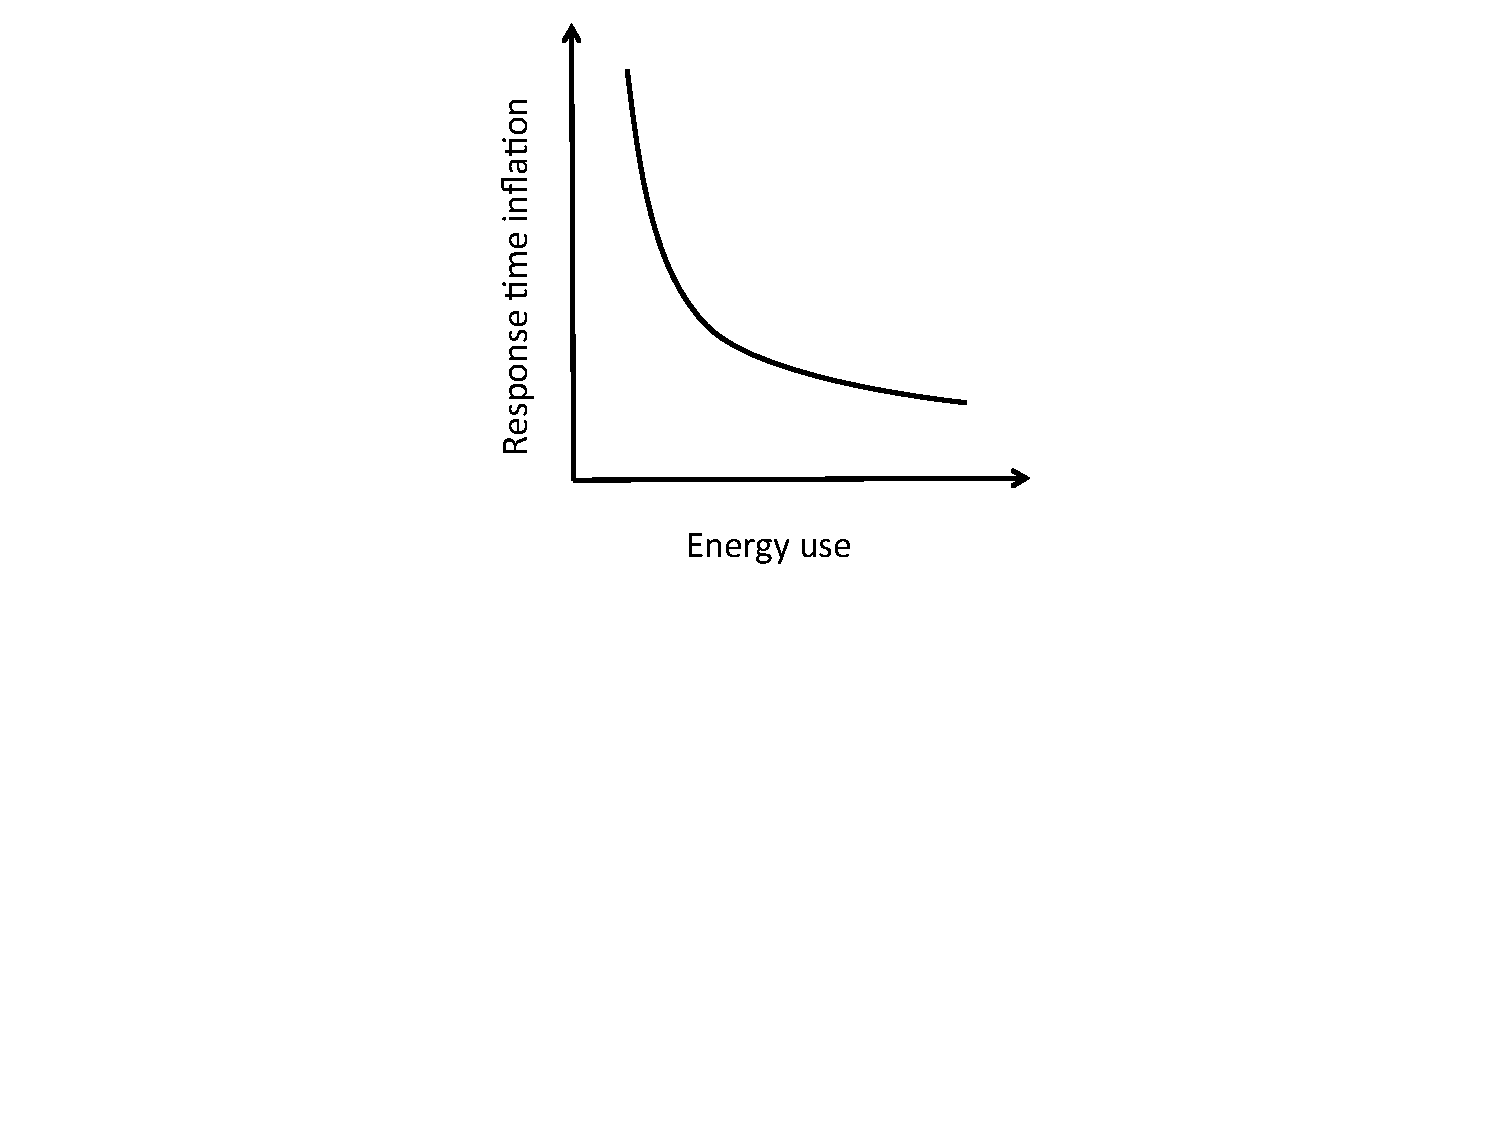
\includegraphics[scale=0.35]{toy-graph.pdf}
%\vspace{-1.5in}
%\caption{An illustration of the tradeoff between energy and performance.}
%\label{fig:toy-graph}
%\end{figure}
%
%The challenge in achieving the above goals simultaneously is that they are often in opposition with each other.  Hence, our work focuses on evaluating the fundamental ways in which the above goals tradeoff with each other. For instance, consider energy efficiency and performance. We illustrate the tradeoff with a  toy example in Figure \ref{fig:toy-graph}. It is easy to maximize performance by keeping entire datacenter always on, but this approach would incur a high energy use. The other extreme approach to maximize energy savings is to completely turn off the entire datacenter at the cost of an infinitely high performance impact. Each \cdc\ may have a different level of tolerance for performance degradation depending on the traffic that it is serving. Thus, our goal is to  quantify the tradeoff and provide a ``knob'' that allows a \cdc\ to operate at its desired point in this tradeoff. 



%\TBD{Can we include a detailed example of energy vs. performance tradeoff?}
\eat{
\subsection{Limitations of prior work}

\begin{figure}
\centering
\vspace{-0.1in}
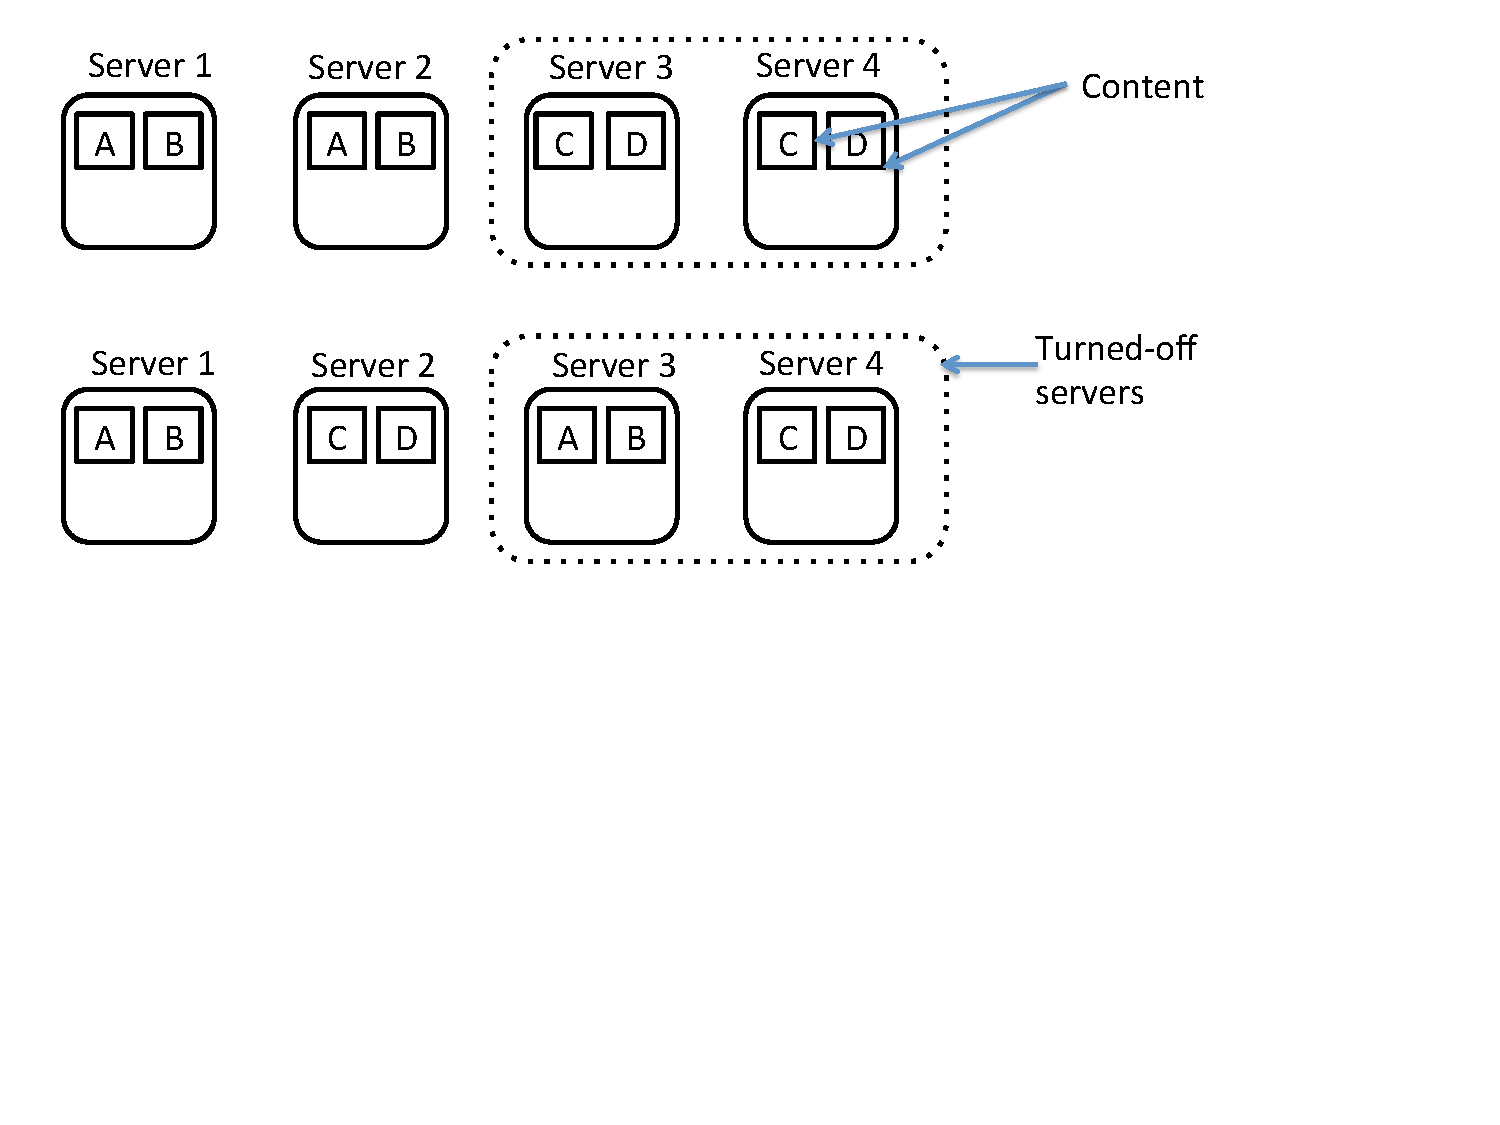
\includegraphics[scale=0.37]{server-content.pdf}
\vspace{-1.5in}
\caption{Content placement must be coordinated with server shutdown to minimize the cache miss rate.}
\label{fig:server-content}
\end{figure}

%Prior efforts at minimizing datacenter energy use have considered  both hardware- and software-level solutions. Hardware-level solutions alone, such as DVFS\cite{henkel2007designing}, leave much room for reducing energy for both servers and switches. Servers have been shown to consume 50-70\% of their peak energy without serving any requests \cite{fan2007power} and networking equipment is even less power proportional and can consume 80-90\% of peak power in idle state \cite{mahadevan2009power}. Software-level solutions reduce energy use by completely turning off components or switching them to a sleep state. For example, server consolidation approaches dynamically adjust the number of active servers based on datacenter load and turn remaining servers off to reduce energy \cite{mathew12,JainEnergy,lin12,lu13}. Similarly, energy-aware routing approaches use only a subset of switches to route traffic and turn off remaining switches  \cite{response, elasticTree, greenTE, Chiaraviglio, Andrews}. 

We describe two key limitations of prior work on server and network consolidation that our work addresses. 

{\em 1)} Prior efforts on server consolidation, including efforts that focus on \cdc s \cite{mathew12, mathew2014energy},  do not account for the fact that different content are stored in the different servers, and further do not explicitly evaluate the impact of the consolidation on response times. However, it is important to devise a load balancer that will coordinate the content placement and server shutdown such that the cache miss rate (and hence response times) does not increase significantly as a result of the shutdown. Consider the example shown in Figure \ref{fig:server-content}. Suppose that all four servers are active during normal utilization periods, but the two servers on the right are turned off during low utilization periods. Squares with same letters represent replicas of the same content. In the top row, content C and D become unavailable within the cluster when servers are turned off, and  an user requesting that content will experience a longer response time as it will have to be refetched from the origin. Whereas in the bottom row one copy of all content is still available within the cluster, resulting in lower response times.

\begin{figure}
\centering
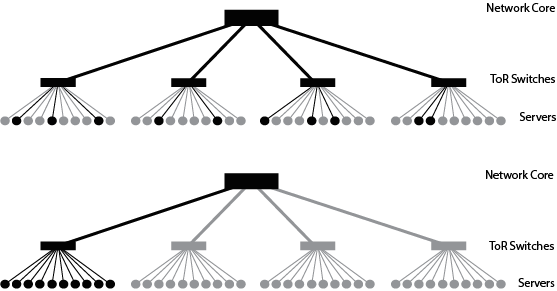
\includegraphics[scale=0.4]{figures/dcTopology.png}
\caption{A datacenter topology. Black (grey) components are turned on (off). 
(Middle) Randomly choosing the set of active servers results in all ToR switches being turned on.
(Bottom) Choosing the same number of active servers in a ``network-aware" manner enables more ToR switches to be turned off.}
\label{fig:server-network}
\end{figure}


{\em 2)} Prior work focus either on server consolidation or network consolidation, but not both. Yet, these problem are closely related as shown in the example in Figure \ref{fig:server-network}. For the same number of active servers, which set of servers is chosen affects potential network energy savings. In the figure, both the middle and the bottom topologies  have the same number of active servers.  The middle topology requires all ToR switches to be kept active, but in the bottom topology the set of active servers are chosen among  servers in one rack which allows ToR switches in other racks to be turned off.  This example shows that network energy minimization is closely related to server energy optimization, and making server consolidation decisions in a network-aware manner can lead to greater energy savings.

\textbf{Summary:} There are two key limitations of prior efforts of energy optimization. First, they do not account for the interaction between server consolidation and load balancing. Second, they treat server and network consolidation as independent problems and hence do not realize the possible energy savings. Addressing these limitations is a key motivation of our work.
}